In statistics, we are given some data $\mathcal{D} = \{x_i\}_{i=1}^n$. The simplest thing we can do is summarize this data by extracting some nice characteristics---for example, the mean. This is known as \textbf{descriptive statistics}. 

In \textbf{inferential statistics}, we have much stronger assumptions. We assume that that data are realizations of random variables following a joint probability distribution. Sometimes, we may assume that these \textbf{samples} are iid coming from $\mathbb{P}^\ast$, known as the \textit{true data generating distribution} (and sometimes known as the \textit{population} in survey statistics or causal inference). As the name suggests, we must infer from $\mathcal{D}$ what $\mathbb{P}$ is. This immediately raises some questions: How should we interpret the population? What are we inferring? And how does this process work? Let's establish this confusion with an example. 

\begin{example}[Measurement Problem]
  Say we have a dataset consisting of real-valued measurements $x_1, \ldots, x_n$ to estimate some quantity $\theta$. We may try to summarize the mean of this data by computing 
  \begin{equation}
    \bar{x} = \frac{x_1 + x_2 + \ldots + x_n}{n} 
  \end{equation} 
  This seems so common and intuitive that we might forget why this specific formula works. Two nice properties are: 
  \begin{enumerate}
    \item It minimizes the sum of least squares 
    \begin{equation}
      \bar{x} = \argmin_{a} \sum_{i=1}^n (x_i - a)^2 
    \end{equation}

    \item The value $\bar{x}$ makes the sum of the residuals to be $0$. 
  \end{enumerate} 
  These two properties land on the level of descriptive statistics. They describe the mean as a reasonable descriptive measure of the center of the observations, but they cannot justify $\bar{x}$ as an estimate of the true value $\theta$ since no explicit assumption has been made connecting the observations $x_i$ with $\theta$. 

  To do inference, we can furthermore assume that the $x_i$ are observed values of $n$ independent random variables which have a common distribution depending on $\theta$. Which assumptions we make will determine which estimators are reasonable. Here are two cases in which means are not a reasonable estimate. 
  \begin{enumerate}
    \item We assume that $x_i = \theta + \epsilon_i$ where $\epsilon_i$ satisfies $\mathbb{P}(\epsilon_i < 0) = \mathbb{P}(\epsilon_i > 0)$. 

    \item \textit{Larger samples may not improve estimate}. If the $x_i$ turns out to have finite variance the variance of the mean is $\sigma^2 /n$. However, if the $x_i$'s have a Cauchy distribution, then the distribution of $\bar{x}$ is the same as $x$, so nothing is gained by taking more measurements. 
  \end{enumerate}
\end{example}

To answer the first question, the population is usually introduced as some finite true distribution of some quantity, but more often it is treated as an abstract data generating distribution. For example, say that we have a large barrel of grains, and we take a random sample of 100 grains and measure their weight. Though we can spend much more effort and time weighing every single grain in the barrel, for practical reasons we want to work with the sample. On the other hand, think of the distribution of facial features of humanity. We may assume that every time a human is born, we can think of it being sampled from some abstract distribution (specified by ``God''), and so even taking all humans in the world is still a sample of this population. 

As for the second and third questions, the general statistical procedure (both frequentist and Bayesian) goes like this.\footnote{Thanks to Ed Tam for giving me such a clear bird's eye view.}
\begin{enumerate}
  \item There exists some true distribution $\mathbb{P}^\ast$ of the population over some \textbf{sample space} $\mathcal{X}$. We want to estimate some (population) \textbf{parameter} $\theta^\ast = T(\mathbb{P}^\ast)$ for some map $T$. This parameter of interest $\theta^\ast$ is called the \textbf{estimand}. 

  There are many types of parameters we can choose from, and generally the form of $T$ can change quite dramatically depending on the type of inference we are doing. 
  \begin{enumerate}
    \item In \textbf{point estimation}, we are interested in vector-valued estimates. For example, the mean $T(\mathbb{P}) = \int x d \mathbb{P}(x)$ is one such candidate. 

    \item In \textbf{hypothesis testing}, we are given a null hypothesis $H_0$, and $T(\mathbb{P}) = \mathbbm{1}_{H_0} (\mathbb{P}) \in \{0, 1\}$. $T$ is therefore a binary function that indicates whether the null hypothesis is true. 

    \item In \textbf{confidence sets}, $T$ is still a point estimate. However, instead of estimating $\theta^\ast$ directly, we construct a set-valued estimator $C_n (\mathcal{D}) \subset \Theta$ designed to contain $\theta^\ast$ with high probability. This is useful for uncertainty quantification. 

    \item In \textbf{density estimation}, $T(\mathbb{P}) = \mathbb{P}$, and we must try to find the distribution $P_\theta$ in our model that best fits $\mathbb{P}^\ast$. 
  \end{enumerate}

  \item We are given a dataset $\mathcal{D} = \{x_i\}_{i=1}^n$ that is sampled from $\mathbb{P}^\ast$. Often, we assume that this is iid. 

  \item We specify a \textbf{model}, which is simply a family of distributions $\mathcal{P} = \{P_{\theta} \mid \theta \in \Theta \}$.\footnote{We may also say a family of functions, but models is more fundamental.} If $\Theta \subset \mathbb{R}^k$, then we say $\mathcal{P}$ is a parameteric family. 

  \item We derive an \textbf{estimator}, which is a function $\delta$ that maps your data to the space that the estimand lives in. The actual value of the function evaluated on your dataset $\hat{\theta} = \delta(\mathcal{D})$ is called the \textbf{estimate}. There are several \textbf{principles} that guide us into deriving such an estimator.\footnote{But none of these principles are frequentist in nature. The key is that frequentism is a way to view probabilities and to view decisions. In other words, it is a way to evaluate things. Principles a to e are often principles that frequentist statisticians use to derive estimators, mainly because such estimators enjoy nice frequentist properties. But none of the methods per se are frequentist in nature. abcd can technically all be lumped under the umbrella of m estimators (although that level of generality and abstractness is seldom useful beyond proof purposes).}
  \begin{enumerate}
    \item \textbf{Maximum Likelihood} estimators attempt to maximize the likelihood $L$ of the data given a model, and so 
    \begin{equation}
      \hat{\theta} = \delta_{MLE}(\mathcal{D}) = \argmax_{\theta} L(\theta \mid \mathcal{D}) 
    \end{equation}

    \item \textbf{Method of Moments} estimators try to match the moments of the model with that of the data. 

    \item \textbf{Score matching} attempt to match the score function---the derivative of the log-likelihood. 

    \item \textbf{M-estimators}. 

    \item \textbf{Minimax estimators}. 
  \end{enumerate}
\end{enumerate}

Next, we talk about model selection, focusing on the cross validation and information criteria. 

\begin{definition}[Empirical Distribution]
  Now given that we have these iid samples, we can construct the \textbf{empirical distribution} $\widehat{X} \sim \widehat{P}$, defined as the discrete distribution that assigns probability $1/n$ to each value $x_i$ for $i \in [n]$. In other words, we have 
  \begin{equation}
    \mathbb{P}(\widehat{X} = x) = \frac{1}{n} \text{ for } x \in \{x_1, \ldots, x_n\}
  \end{equation}
  We can write the CDF of the empirical distribution, called the \textbf{empirical distribution function}, as the sum of indicators
  \begin{equation}
    F_X (x) = \frac{1}{n} \sum_{i=1}^n \mathbb{I}_{[x_i, +\infty)} (x)
  \end{equation}
\end{definition}

As expected, we would expect the empirical distribution to converge to the actual distribution. 

\begin{theorem}[Glivenko–Cantelli theorem]
  The empirical distribution of iid samples $x_1, \ldots, x_n \sim P_n$ converges almost surely to $X \sim P$ as $n \rightarrow \infty$. More specifically, given that the CDF of $X$ is $F$ and the CDF of $P_n$ is the step function $F_n$, we have 
  \begin{equation}
    ||F_n - F||_{\infty} = \sup_{x \in \mathbb{R}} |F_n (x) - F(x)| \rightarrow 0
  \end{equation}
  almost surely as $n \rightarrow \infty$. 
\end{theorem}

\begin{example}[Empirical Distribution of Standard Gaussian]
  We expect the empirical distribution of the standard Gaussian to converge. Indeed, numerical results show that for 10 and 100 samples, the empirical CDF does converge to the true CDF. 

  \begin{center}
    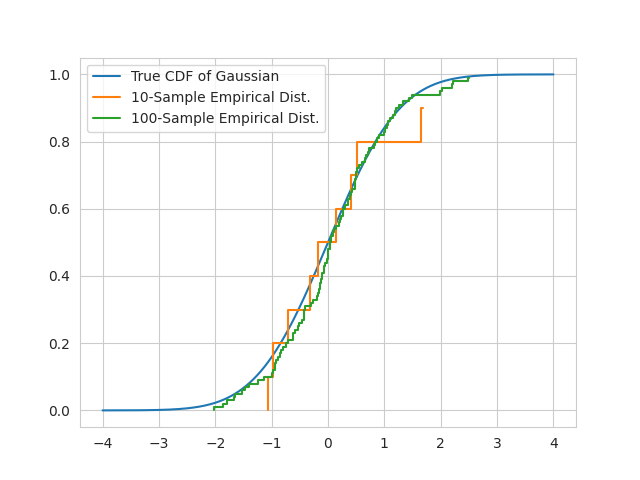
\includegraphics[scale=0.4]{img/empirical_distribution.png}
  \end{center}
\end{example}


